\documentclass[]{article}
\usepackage{lmodern}
\usepackage{amssymb,amsmath}
\usepackage{ifxetex,ifluatex}
\usepackage{fixltx2e} % provides \textsubscript
\ifnum 0\ifxetex 1\fi\ifluatex 1\fi=0 % if pdftex
  \usepackage[T1]{fontenc}
  \usepackage[utf8]{inputenc}
\else % if luatex or xelatex
  \ifxetex
    \usepackage{mathspec}
  \else
    \usepackage{fontspec}
  \fi
  \defaultfontfeatures{Ligatures=TeX,Scale=MatchLowercase}
\fi
% use upquote if available, for straight quotes in verbatim environments
\IfFileExists{upquote.sty}{\usepackage{upquote}}{}
% use microtype if available
\IfFileExists{microtype.sty}{%
\usepackage{microtype}
\UseMicrotypeSet[protrusion]{basicmath} % disable protrusion for tt fonts
}{}
\usepackage[margin=1in]{geometry}
\usepackage{hyperref}
\hypersetup{unicode=true,
            pdftitle={Sequential Stein Variational Gradient Descent for Time Series Model Estimation},
            pdfauthor={Gibson, Reich, and Ray in some order},
            pdfborder={0 0 0},
            breaklinks=true}
\urlstyle{same}  % don't use monospace font for urls
\usepackage{graphicx,grffile}
\makeatletter
\def\maxwidth{\ifdim\Gin@nat@width>\linewidth\linewidth\else\Gin@nat@width\fi}
\def\maxheight{\ifdim\Gin@nat@height>\textheight\textheight\else\Gin@nat@height\fi}
\makeatother
% Scale images if necessary, so that they will not overflow the page
% margins by default, and it is still possible to overwrite the defaults
% using explicit options in \includegraphics[width, height, ...]{}
\setkeys{Gin}{width=\maxwidth,height=\maxheight,keepaspectratio}
\IfFileExists{parskip.sty}{%
\usepackage{parskip}
}{% else
\setlength{\parindent}{0pt}
\setlength{\parskip}{6pt plus 2pt minus 1pt}
}
\setlength{\emergencystretch}{3em}  % prevent overfull lines
\providecommand{\tightlist}{%
  \setlength{\itemsep}{0pt}\setlength{\parskip}{0pt}}
\setcounter{secnumdepth}{0}
% Redefines (sub)paragraphs to behave more like sections
\ifx\paragraph\undefined\else
\let\oldparagraph\paragraph
\renewcommand{\paragraph}[1]{\oldparagraph{#1}\mbox{}}
\fi
\ifx\subparagraph\undefined\else
\let\oldsubparagraph\subparagraph
\renewcommand{\subparagraph}[1]{\oldsubparagraph{#1}\mbox{}}
\fi

%%% Use protect on footnotes to avoid problems with footnotes in titles
\let\rmarkdownfootnote\footnote%
\def\footnote{\protect\rmarkdownfootnote}

%%% Change title format to be more compact
\usepackage{titling}

% Create subtitle command for use in maketitle
\newcommand{\subtitle}[1]{
  \posttitle{
    \begin{center}\large#1\end{center}
    }
}

\setlength{\droptitle}{-2em}
  \title{Sequential Stein Variational Gradient Descent for Time Series Model
Estimation}
  \pretitle{\vspace{\droptitle}\centering\huge}
  \posttitle{\par}
  \author{Gibson, Reich, and Ray in some order}
  \preauthor{\centering\large\emph}
  \postauthor{\par}
  \predate{\centering\large\emph}
  \postdate{\par}
  \date{December 3, 2017}

\usepackage{multicol}
\usepackage{amssymb}
\usepackage{amsmath}

\begin{document}
\maketitle

\section{Introduction}\label{introduction}

Particle filtering suffers from two main practical disadvantages. The
first is particle depletion, where the number of effective particles
with non-neglibile weight becomes too small. This has the effect of
concentrating the mass around a small number of particles, leading to
poor estimates of the target distribution. The second is the running
time of the algorithm. A cursory analysis reveals that each particle is
updated once per time step in the time series, and once per re-sampling
step, to mitigate the issue above. If we imagine the order of particles
is close to the length of the time series, we see that run-time is
\(O(n^3)\).

We propose another approach that we hope will do better than particle
filtering in practice. In this approach, Stein Variational Gradient
Descent (SVGD) is used to sequentially estimate the distribution of
state variables in each time step, conditional on observed data up
through that time. This method should overcome problems with particle
depletion and excessive run-times for long time-series.

\subsection{Overview of SVGD}\label{overview-of-svgd}

Stein Variational Gradient Descent can be used to estimate a continuous
distribution by a set of samples. By iteratively transporting samples
from an initial distribution in the direction of the likelihood, we are
able to generate a sample from the target distribution. The usefullness
of this approximation is apparent in Bayesian statistics, where the
usually intractable normalizing constant disappears in the gradient. The
particles are subject to the following gradient ascent procedure.

\[x_t^{(i)} \leftarrow x_{t-1}^{(i)} + \frac{1}{n}\sum_{j=1}^n[ k(x_j,x_{t-1}^{(i)})*\nabla log\ p(x_j) + \nabla k(x_j,,x_{t-1}^{(i)})]\]

\subsection{Sequential Stein Variational Gradient
Descent}\label{sequential-stein-variational-gradient-descent}

Suppose we are given a time series \(Y_1,Y_2,...,Y_t\) for
\(Y \in \mathbb{R}\). We model the sequence as a state-space model
parameterized by an observation density \(p(y_t | x_t)\) and a
transition density \(p(x_t | x_{t-1})\) Figure 1.

\begin{figure}[htbp]
\centering
\includegraphics{/Users/gcgibson/Desktop/ssm.png}
\caption{Caption for the picture.}
\end{figure}

We are interested in the filtering distribution
\(p(x_1,...,x_n | y_1,...,y_n)\) which by Bayes formula is
\[p(x_1,...,x_n | y_1,...,y_n) = \frac{p(y_1,...,y_n | x_1,...,x_n) p(x_1,...,x_n)}{Z}\].

Because computing the normalizing constant \(Z\) is intractable for many
choices of \(p(y_t | x_t)\) and \(p(x_t | x_{t-1})\), we must resort to
monte carlo algorithms. The classic approach that incorporates the
sequential nature of the data is given by the particle filtering
algorithm. Particle filtering approximates the filtering density using
sequential importance sampling. We instead focus on the following
recursion.

\[p(x_t | y_{1:t}) = \int p(x_{0:t} | y_{1:t})d_{x_0:t-1}\]
\[=\frac{p(y_t | x_t)}{\int p(y_t|x_t)p(x_t | y_{1:t-1})dx_t}p(x_t | y_{1:t-1})\]

\[\propto p(y_t|x_t)p(x_t | y_{1:t-1})\]
\[\propto p(y_t|x_t)p(x_t | y_{1:t-1})\]
\[\propto p(y_t|x_t)\int_{x_{t-1}}p(x_t,x_{t-1} | y_{1:t-1})d_{x_{t-1}}\]

\[\propto p(y_t|x_t)\int_{x_{t-1}}p(x_t |x_{t-1} )p(x_{t-1}| y_{1:t-1})d_{x_{t-1}}\]

which we can approximate using svgd as
\[\approx p(y_t|x_t) \frac{1}{n}\sum_{i=1}^n p(x_t | x_{t-1}^{(i)})\] We
can now estimate \(p(x_{t+1}|y_{1:t+1})\) using the same algebra as
above. (proof in apendix A)

\subsection{Model Structure}\label{model-structure}

States:

\begin{itemize}
\item $X_1 \sim g_1(x_1 ; \xi)$
\item $X_t \vert X_{t-1} \sim g(x_t \vert x_{t - 1} ; \xi)$ for all $t = 2, \ldots, T$
\end{itemize}

Observations:

\begin{itemize}
\item $Y_t \vert X_{t} \sim h(y_t | x_t ; \zeta)$
\end{itemize}

Here, \(g_1(\cdot)\) and \(g(\cdot)\) are appropriately defined
probability density functions depending on parameters \(\xi\) and
\(h(\cdot)\) is an appropriately defined probability density function or
probability mass function depending on parameters \(\zeta\).

Define \(\theta = (\xi, \zeta)\) to be the full set of model parameters.

\subsection{Filtering}\label{filtering}

There are two types of filtering:

\begin{enumerate}
\def\labelenumi{\arabic{enumi}.}
\tightlist
\item
  sample of particles \(x_{1:T}^{(k)} \sim f(x_{1:T} | y_{1:T})\)
\item
  sample of particles \(x_{t}^{(k)} \sim f(x_{t} | y_{1:t})\) for each
  \(t = 1, \ldots, T\)
\end{enumerate}

Let's look at the second one. Assume we have a sample
\(x_{t-1}^{(k)} \sim f(x_{t-1} | y_{1:t-1})\)

\begin{align*}
p(x_{t} | y_{1:t}) &= \frac{f(x_t, y_t | y_{1:t-1})}{f(y_t | y_{1:t-1})} \\
 &\propto f(x_t, y_t | y_{1:t-1}) \\
 &= f(y_t | x_t) f(x_t | y_{1:t-1}) \\
 &= f(y_t | x_t) \int f(x_t, x_{t-1} | y_{1:t-1}) d x_{t-1} \\
 &= f(y_t | x_t) \int f(x_t | x_{t - 1}) f(x_{t-1} | y_{1:{t-1}}) dx_{t-1} \\
 &\approx f(y_t | x_t) \sum_{x_{t-1}^{(k)}} f(x_t | x_{t - 1}^{(k)})
\end{align*}

So \(\log\{p(x_{t} | y_{1:t})\}\) is approximately proportional to
\(\log\{f(y_t | x_t)\} + \log\{\sum_{x_{t-1}^{(k)}} f(x_t | x_{t - 1}^{(k)})\}\)

\subsection{Locally Level Gaussian Noise
Model}\label{locally-level-gaussian-noise-model}

In order to demonstrate that the approximation is reasonable we evaluate
the predictive accuracy under an analytically tractable model, the
locally level Gaussian model. This model takes the form
\[X_t \sim N(X_{t-1},\sigma_1^2)\] \[Y_t \sim N(X_t, \sigma_2^2)\]

\begin{verbatim}
## 
## Attaching package: 'dlm'
\end{verbatim}

\begin{verbatim}
## The following object is masked from 'package:ggplot2':
## 
##     %+%
\end{verbatim}

\begin{verbatim}
## [1] "python /Users/gcgibson/Stein-Variational-Gradient-Descent/python/locally_level_gaussian.py  0.285676619609561, 2.91753012580183, 2.78117622763953, 4.69683824157547, 5.74877016964816, 3.57537019527663, 7.39631203226068, 6.22488628594129, 7.82768183893382, 11.6222569023377"
\end{verbatim}

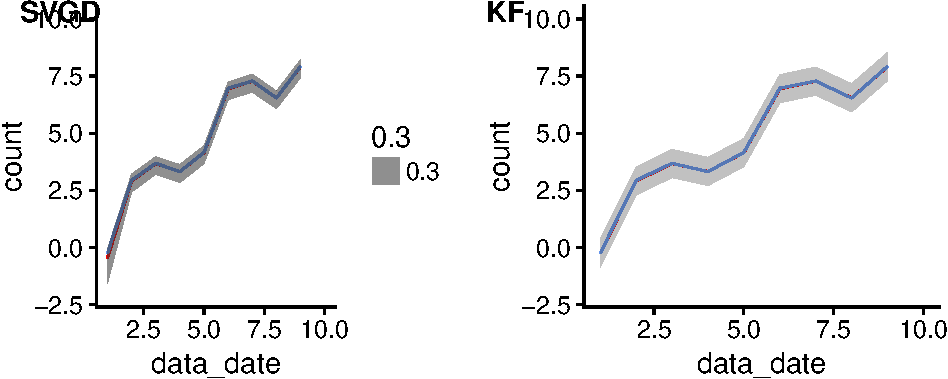
\includegraphics{ssvgd_files/figure-latex/unnamed-chunk-2-1.pdf}
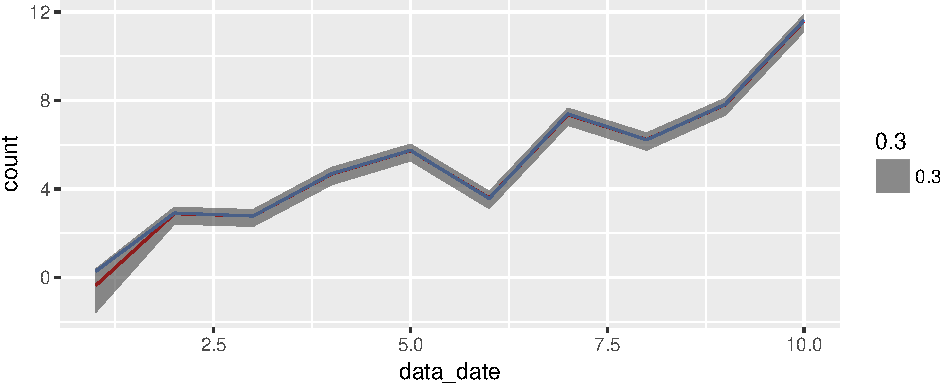
\includegraphics{ssvgd_files/figure-latex/unnamed-chunk-2-2.pdf}

\begin{verbatim}
## Warning: package 'cowplot' was built under R version 3.4.3
\end{verbatim}

\begin{verbatim}
## 
## Attaching package: 'cowplot'
\end{verbatim}

\begin{verbatim}
## The following object is masked from 'package:ggplot2':
## 
##     ggsave
\end{verbatim}

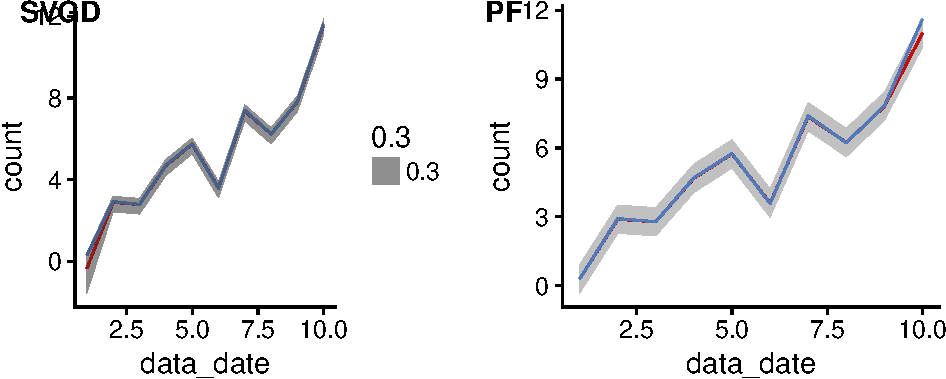
\includegraphics{ssvgd_files/figure-latex/unnamed-chunk-2-3.pdf}

\subsection{Poisson Observation Model With Seasonal State-Space
Dynamics}\label{poisson-observation-model-with-seasonal-state-space-dynamics}

In order to evaluate the performance on more involved dynamics we
consider the following state-space model.
\[\begin{pmatrix} X_{t,1} \\ X_{t,2} \end{pmatrix} = \begin{pmatrix} cos(2\pi/s) & sin(2\pi/s) \\ -sin(2\pi/s) & cos(2\pi/s) \end{pmatrix} \begin{pmatrix} X_{t-1,1} \\ X_{t-1,2} \end{pmatrix} \]
\[Y_t \sim Pois(e^{X_{t,1}})\]

\begin{verbatim}
## Loading required package: rbiips
\end{verbatim}

\begin{verbatim}
## Loading required package: coda
\end{verbatim}

\begin{verbatim}
## Loading required package: MASS
\end{verbatim}

\begin{verbatim}
## 
## Attaching package: 'MASS'
\end{verbatim}

\begin{verbatim}
## The following object is masked from 'package:dplyr':
## 
##     select
\end{verbatim}

\begin{verbatim}
## ##
## ## Markov Chain Monte Carlo Package (MCMCpack)
\end{verbatim}

\begin{verbatim}
## ## Copyright (C) 2003-2018 Andrew D. Martin, Kevin M. Quinn, and Jong Hee Park
\end{verbatim}

\begin{verbatim}
## ##
## ## Support provided by the U.S. National Science Foundation
\end{verbatim}

\begin{verbatim}
## ## (Grants SES-0350646 and SES-0350613)
## ##
\end{verbatim}

\begin{verbatim}
## * Parsing model in: /Users/gcgibson/Stein-Variational-Gradient-Descent/bug_files/seasonal_pois.bug
\end{verbatim}

\begin{verbatim}
## Warning in biips_model(seasonal_model_file, data = seasonal_data,
## sample_data = FALSE): Unused variables in data: G, mean_sigma_init,
## cov_sigma_init, mean_x_init
\end{verbatim}

\begin{verbatim}
## * Compiling model graph
##   Declaring variables
##   Resolving undeclared variables
##   Allocating nodes
##   Graph size: 121
\end{verbatim}

\begin{verbatim}
## * Assigning node samplers
## * Running SMC forward sampler with 100000 particles
##   |--------------------------------------------------| 100%
##   |**************************************************| 11 iterations in 20.80 s
\end{verbatim}

\begin{verbatim}
## [1] "python /Users/gcgibson/Stein-Variational-Gradient-Descent/python/seasonal.py  17, 18, 10, 16, 19, 11, 14, 20, 12, 13"
\end{verbatim}

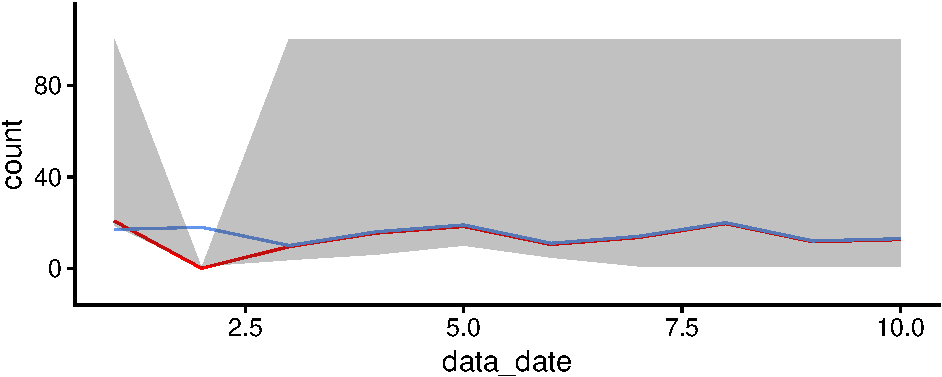
\includegraphics{ssvgd_files/figure-latex/unnamed-chunk-3-1.pdf}
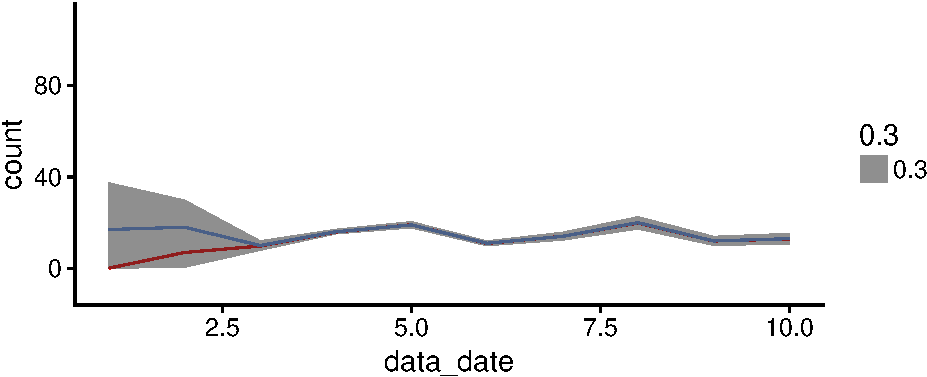
\includegraphics{ssvgd_files/figure-latex/unnamed-chunk-3-2.pdf}
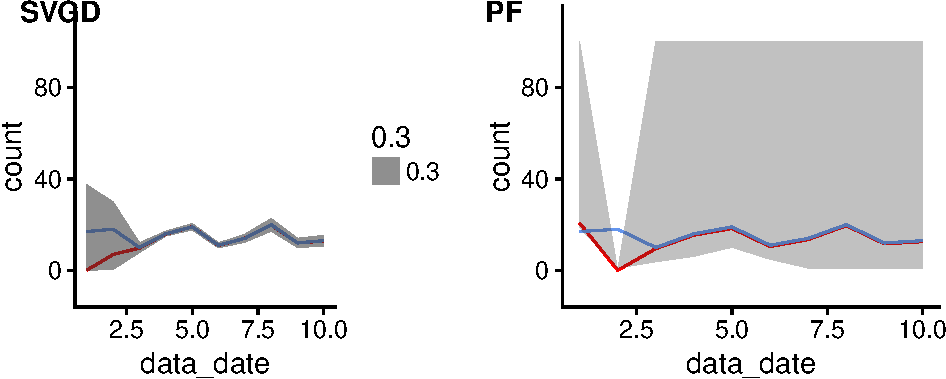
\includegraphics{ssvgd_files/figure-latex/unnamed-chunk-3-3.pdf}

\subsection{Divergent Particle Filter}\label{divergent-particle-filter}

We next investigate the ability of SSVGD to perform in the presence of
poor initialization. This is a well known issue with current particle
filter implemntations: starting far from a plausabile value of \(x_0\)
forces all particles to receive weight \(0\) under the likelihood,
leading to a degenerate filtering distribution. However, under SSVGD, we
can simply increase the number of iterations, allowing for arbitrarily
poor starting points.

\begin{verbatim}
## * Parsing model in: /Users/gcgibson/Stein-Variational-Gradient-Descent/bug_files/locally_level_1.bug
## * Compiling model graph
##   Declaring variables
##   Resolving undeclared variables
##   Allocating nodes
##   Graph size: 18
\end{verbatim}

\begin{verbatim}
## * Assigning node samplers
## * Running SMC forward sampler with 10000 particles
##   |--------------------------------------------------| 100%
##   |**************************************************| 5 iterations in 0.24 s
\end{verbatim}

\begin{verbatim}
## * Diagnosis of variable: x[1:5] 
##   Filtering: POOR
##     The minimum effective sample size is too low: 8.788576 
##     Estimates may be poor for some variables.
##     You should increase the number of particles
## .  Smoothing: POOR
##     The minimum effective sample size is too low: 3.664264 
##     Estimates may be poor for some variables.
##     You should increase the number of particles
## .
\end{verbatim}

\begin{verbatim}
## [1] 0.0001262422 0.0115295532 0.0112004317 0.6160331587 1.2560522188
\end{verbatim}

\begin{verbatim}
## [1] "python /Users/gcgibson/Stein-Variational-Gradient-Descent/python/locally_level.py  1, 4, 0, 3, 2"
\end{verbatim}

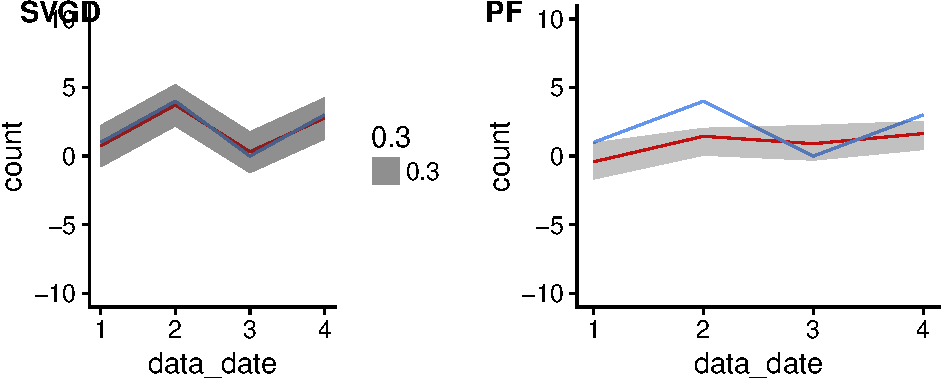
\includegraphics{ssvgd_files/figure-latex/unnamed-chunk-4-1.pdf}
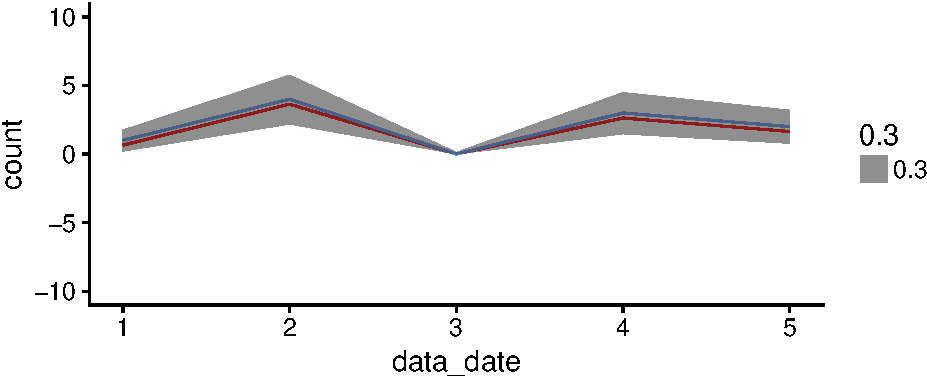
\includegraphics{ssvgd_files/figure-latex/unnamed-chunk-4-2.pdf}
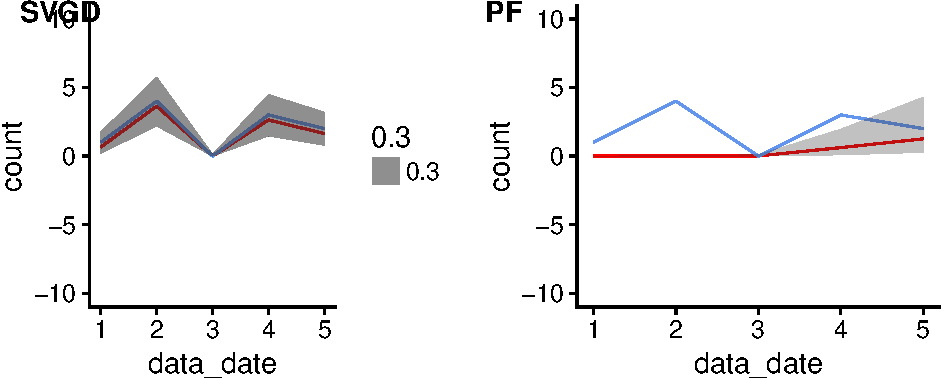
\includegraphics{ssvgd_files/figure-latex/unnamed-chunk-4-3.pdf}

\paragraph{Results}\label{results}

Paragraph, referencing one figure and one table, summarizing results

\subsection{Application}\label{application}

Example model with real data. fairly real model, but not thaaaaaat
complex.

\subsection{Discussion}\label{discussion}

\subsection{Bibliography}\label{bibliography}


\end{document}
